\section{Raft overview}
\label{basicraft:overview}

\begin{figure*}
\centering
\includegraphics[scale=0.95]{basicraft/cheatsheet}
\vcaption[algorithm summary]{
A condensed summary of the \name{} consensus algorithm (excluding
membership changes, log compaction, and client interaction).
The server behavior in the
lower-right box is described as a set of rules that trigger independently
and repeatedly.
Section numbers such as \S\ref{basicraft:leaderelection} indicate where particular features
are discussed. The formal specification in
Appendix~\ref{appendix:correctness} describes the
algorithm more precisely.
}
\label{fig:basicraft:cheatsheet}
\end{figure*}


\begin{figure}
\centering
\fbox {
  \parbox{5.1in}{
    \small
    \begin{description}
    \itemsep 0em
    \item[\textbf{Election Safety}] \hfill \\
    At most one leader can be elected in
    a given term.
    \S\ref{basicraft:leaderelection}

    \item[\textbf{Leader Append-Only}] \hfill \\
    A leader never overwrites or deletes
    entries in its log; it only appends new entries. \S\ref{basicraft:logreplication}

    \item[\textbf{Log Matching}] \hfill \\
    If two logs contain an entry with
    the same index and term, then the logs are identical in all entries
    up through the given index. \S\ref{basicraft:logreplication}

    \item[\textbf{Leader Completeness}] \hfill \\
    If a log entry is committed
    in a given term, then that entry will be present in the logs of
    the leaders for all higher-numbered terms.
    \S\ref{basicraft:safety}

    \item[\textbf{State Machine Safety}] \hfill \\
    If a server has applied a
    log entry at a given index to its state machine, no other server
    will ever apply a different log entry for the same index.
    \S\ref{basicraft:safety:argument}
    \vspace{-0.5ex}
    \end{description}
  }
}
\vcaption[key properties]{
\name{} guarantees that each of these properties is true at all times. The
section numbers indicate where each property is discussed.
}
\label{fig:basicraft:properties}
\end{figure}


Raft is an algorithm for managing
a replicated log of the form described in Section~\ref{motivation:problem}.
Figure~\ref{fig:basicraft:cheatsheet}
summarizes the algorithm in condensed form for reference,
and Figure~\ref{fig:basicraft:properties} lists key properties of the
algorithm; the elements of these figures
are discussed piecewise over the rest of this chapter.

\name{} implements consensus by first electing a server as
\emph{leader}, then giving
the leader complete responsibility for managing the replicated log. The leader
accepts log entries from clients, replicates them on other servers, and
tells servers when it is safe to apply log entries to their state machines.
Having a leader simplifies the management of the replicated log. For
example, the leader can decide where to place new entries in the log without
consulting other servers, and data flows in a simple fashion from
the leader to other servers.
A leader can fail or become disconnected from the other servers, in which
case a new leader is elected.

Given the leader approach, \name{} decomposes the consensus problem
into three relatively independent subproblems, which are discussed
in the subsections that follow:
\begin{itemize}
    \item \textbf{Leader election:} a new leader must be chosen
    when starting the cluster and when
    an existing leader fails (Section~\ref{basicraft:leaderelection}).
    \item \textbf{Log replication:} the leader must accept log entries
    from clients and replicate them across the cluster,
    forcing the other logs to agree with its own
    (Section~\ref{basicraft:logreplication}).
    \item \textbf{Safety:} the key safety property for \name{} is the
    State Machine Safety Property in Figure~\ref{fig:basicraft:properties}: if any
    server has applied a particular log entry to its state machine,
    then no other server may apply a different command for the
    same log index. Section~\ref{basicraft:safety} describes
    how \name{} ensures this property; the solution involves
    an additional restriction on the election mechanism described
    in Section~\ref{basicraft:leaderelection}.
\end{itemize}
After presenting the consensus algorithm, this chapter discusses the
issue of availability and the role of timing in the system
(Section~\ref{basicraft:timing}), and an optional extension to transfer
leadership between servers (Section~\ref{basicraft:leadershiptransfer}).

\section{\name{} basics}
\label{basicraft:basics}

A \name{} cluster contains several servers; five is a typical
number, which allows the system to tolerate two failures.
At any given time each server is in one of three states: \emph{leader},
\emph{follower}, or \emph{candidate}. In normal operation there is
exactly one leader and all of the other servers are followers. Followers
are passive: they issue no requests on their own but simply
respond to requests from leaders and candidates. The leader handles all
client requests (if a client contacts a
follower, the follower redirects it to the leader).
The third state, candidate, is used to elect a new leader as
described in Section~\ref{basicraft:leaderelection}.
Figure~\ref{fig:basicraft:followercandidateleader} shows the states and
their transitions; the transitions are discussed
below.

\name{} divides time into \emph{terms} of arbitrary length,
as shown in Figure~\ref{fig:basicraft:terms}.
Terms are numbered with consecutive integers. Each term begins with an
\emph{election}, in which one or more candidates attempt to become
leader as described in Section~\ref{basicraft:leaderelection}. If a candidate
wins the election, then it serves as
leader for the rest of the term. In some situations an election will
result in a split vote. In this case the
term will end with no leader; a new term (with a new election)
will begin shortly. \name{} ensures that there is at most one leader
in a given term.
\begin{figure}
\centering
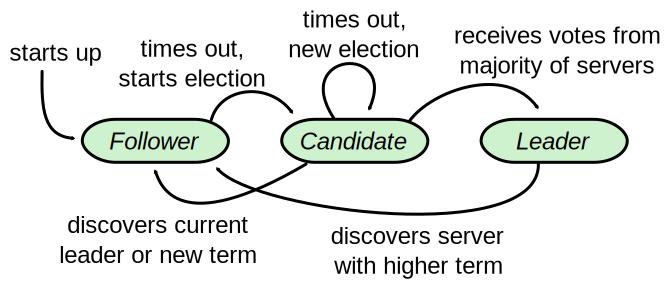
\includegraphics[scale=.50]{basicraft/followercandidateleader}
\vcaption[server states]{
Server states. Followers only respond to
requests from other servers. If a follower receives no communication, 
it becomes a candidate and initiates an election. A candidate
that receives votes from a majority of the full cluster becomes the new
leader. Leaders typically operate until they fail.}
\label{fig:basicraft:followercandidateleader}
\end{figure}

\begin{figure}
\centering
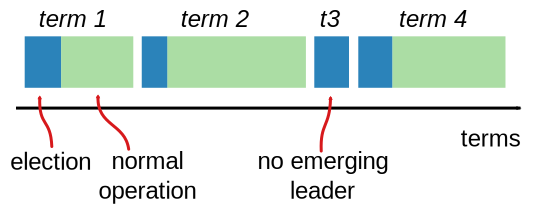
\includegraphics[scale=.50]{basicraft/terms}
\vcaption[terms]{
Time is divided into terms, and each term begins with an election. After
a successful election, a single leader manages the cluster until the end
of the term. Some elections fail, in which case the term ends without
choosing a leader.
The transitions between terms may be observed at different times on
different servers. 
}
\label{fig:basicraft:terms}
\end{figure}

Different servers may observe the transitions between terms
at different times, and in some situations a server may not observe
an election or even entire terms.
Terms act as a logical clock~\cite{Lamport:1978} in \name{},
and they allow
servers to detect obsolete information such as stale leaders.
Each server stores a \emph{current term} number, which increases
monotonically over time. Current terms are exchanged whenever
servers communicate; if one server's current term is smaller than
the other's, then it updates its current term to the larger value.
If a candidate or leader discovers that its term is out of date,
it immediately reverts to follower state.
If a server receives a request with a stale term number, it
rejects the request.

Raft servers communicate using remote procedure calls (RPCs), and the
basic consensus algorithm requires only two types of RPCs between
servers. RequestVote RPCs are initiated by candidates during elections
(Section~\ref{basicraft:leaderelection}), and AppendEntries RPCs are
initiated by leaders to replicate log entries and to provide a form of
heartbeat (Section~\ref{basicraft:logreplication}). Leadership transfer
(Section~\ref{basicraft:leadershiptransfer}) and the mechanisms
described in subsequent chapters introduce additional RPCs beyond the
two in the core consensus algorithm.

We chose to structure communication in Raft as RPCs to simplify
its communication patterns. Each request type has a corresponding response
type, which also serves as the request's acknowledgment. Raft assumes RPC
requests and responses may be lost in the network; it is the requester's
responsibility to retry the RPC if it does not receive a response in a
timely manner. Servers issue RPCs in parallel for best performance, and
Raft does not assume the network preserves ordering between RPCs.

\section{Leader election}
\label{basicraft:leaderelection}

\name{} uses a heartbeat mechanism to trigger leader election.
When servers start up, they begin
as followers. A server remains in follower state as long as it
receives valid RPCs from a leader or candidate. Leaders send periodic
heartbeats (AppendEntries RPCs that carry no log entries) to all
followers in order to maintain their authority. If a follower
receives no communication over a
period of time called the \emph{election timeout}, then
it assumes there is no viable leader and
begins an election to choose a new leader.



To begin an election, a follower increments its current term and
transitions to candidate state. It then votes for itself and issues RequestVote RPCs in
parallel to each of the other servers in the cluster.
A candidate continues in this state until one of three things
happens: (a) it wins the election, (b) another server establishes
itself as leader, or (c) another
election timeout goes by with no winner.
These outcomes are discussed separately in the paragraphs below.

A candidate wins an election if it receives votes from a majority
of the servers in the full cluster for the same term. Each server will
vote for at most one candidate in a given term, on a
first-come-first-served basis (note: Section~\ref{basicraft:safety} adds
an additional restriction on votes). The
majority rule ensures that at most one candidate can win
the election for a particular term (the Election Safety Property
in Figure~\ref{fig:basicraft:properties}).
Once a candidate wins an election, it becomes leader.
It then sends heartbeat messages to
all of the other servers to establish its authority and prevent new elections.

While waiting for votes, a candidate may receive an AppendEntries RPC
from another server claiming to be leader. If the leader's term
(included in its RPC) is at least as large as the candidate's
current term, then the candidate recognizes the leader as legitimate
and returns to follower state.
If the term in the RPC is smaller than the candidate's current term,
then the candidate rejects the RPC and continues in candidate state.

The third possible outcome is that a candidate neither wins nor loses
the election:
if many followers become candidates at the same time, votes could be
split so that no candidate obtains a majority. When this happens,
each candidate will time out and start
a new election by incrementing its term and initiating another round
of RequestVote RPCs. However, without extra measures
split votes could repeat indefinitely.

\name{} uses randomized election timeouts to ensure that split votes
are rare and that they are resolved quickly. To prevent split
votes in the first place, election timeouts are chosen randomly
from a fixed interval (e.g., \SIrange{150}{300}{\milli\second}).
This spreads out the servers
so that in most cases only a single server will time out; it wins the
election and sends heartbeats before any other servers time out.
The same mechanism is used to handle split votes. Each candidate
restarts its randomized election timeout at the start of an election,
and it waits for that timeout to elapse before starting the
next election; this reduces the likelihood of
another split vote in the new election.
Chapter~\ref{leaderelection} shows that this approach
elects a leader rapidly.


Elections are an example of how understandability guided
our choice between design alternatives. Initially we planned to use
a ranking system: each candidate was assigned a unique
rank, which was used to select between competing candidates.
If a candidate discovered another candidate with higher
rank, it would return to follower state so that the
higher ranking candidate could more easily win the next election.
We found that this approach
created subtle issues around availability
(a lower-ranked server might need to time out and become a
candidate again if a higher-ranked server fails, but if it does so too
soon, it can reset progress towards electing a leader).
We made adjustments to the algorithm
several times, but after each adjustment new corner cases appeared.
Eventually we concluded that the randomized retry approach is more
obvious and understandable.

\section{Log replication}
\label{basicraft:logreplication}

Once a leader has been elected, it begins servicing client requests.
Each client request contains a
command to be executed by the replicated state machine.
The leader appends the command to its log as a new entry, then issues
AppendEntries RPCs in parallel to each of the other servers to
replicate the entry.
When the entry has been safely replicated (as described below),
the leader
applies the entry to its state machine and
returns the result of
that execution to the client. If followers crash or run slowly, or
if network packets are lost, the leader retries AppendEntries RPCs
indefinitely (even after it has responded to the client)
until all followers eventually store all log entries.

\begin{figure}
\centering
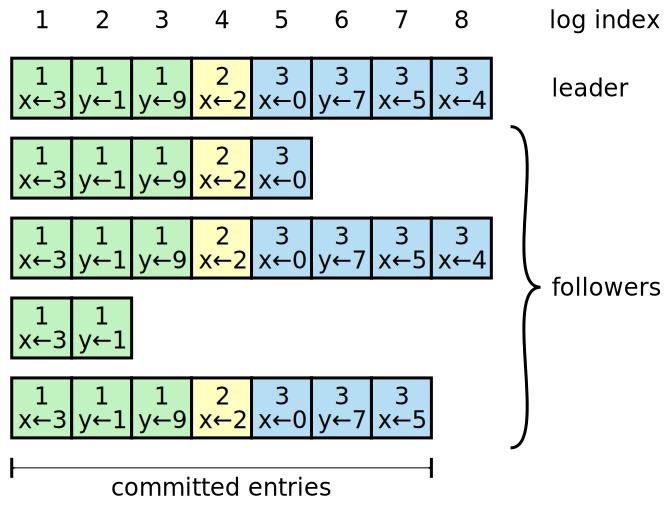
\includegraphics[scale=.50]{basicraft/log2}
\vcaption[log structure]{
Logs are composed of entries, which are numbered sequentially. Each
entry contains the term in which it was created (the number in each
box) and a command for the state machine. An entry is considered
\emph{committed} if it is safe for that entry to be applied to
state machines.}
\label{fig:basicraft:log}
\end{figure}

Logs are organized as shown in Figure~\ref{fig:basicraft:log}.
Each log entry stores a state machine command along with the
term number when the entry was received by the leader.
The term numbers in log entries are used to detect inconsistencies
between logs and to ensure some of the properties in
Figure~\ref{fig:basicraft:properties}. Each log entry
also has an integer index identifying its position in the log.

The leader decides when it is safe to apply a log entry to the
state machines; such an entry is called \emph{committed}.
\name{} guarantees that committed entries are durable
and will eventually be executed by all of the available state machines.
A log entry is committed once the leader that created the
entry has replicated it on a majority of the servers
(e.g., entry 7 in Figure~\ref{fig:basicraft:log}). 
This also commits all preceding entries in the leader's log, including
entries created by previous leaders.
Section~\ref{basicraft:safety} discusses some subtleties when applying
this rule after leader changes, and it also shows
that this definition of commitment is safe.
The leader keeps track of the highest index
it knows to be committed, and it includes
that index in future AppendEntries RPCs (including heartbeats) so
that the other servers eventually find out. Once a follower
learns that a log entry is committed, it applies the entry
to its local state machine (in log order).

We designed the \name{} log mechanism to maintain a high level
of coherency between the logs on different servers. Not only does this
simplify the system's behavior and make it more predictable,
but it is an important component of ensuring safety.
\name{} maintains
the following properties,
which together constitute the Log Matching Property in
Figure~\ref{fig:basicraft:properties}:
\begin{compactitem}
\item If two entries in different logs have the same index and term,
then they store the same command.
\item If two entries in different logs have the same index and term,
then the logs are identical in all preceding entries.
\end{compactitem}

The first property follows from the fact
that a leader creates at most one entry with a given log index
in a given term, and log entries never change their position in
the log.
The second property is guaranteed by a consistency check
performed by AppendEntries. When sending an AppendEntries RPC,
the leader
includes the index and term of the entry in its log that immediately
precedes the new entries.
If the follower does not find an entry in its log with the same
index and term, then it refuses the new entries.
The consistency check acts as an induction step: the
initial empty state of the logs satisfies the
Log Matching Property,
and the consistency check preserves the
Log Matching Property whenever logs are
extended. As a result, whenever AppendEntries returns successfully,
the leader knows that the follower's log is identical to its own log
up through the new entries.

During normal operation, the logs of the leader and followers stay
consistent, so the AppendEntries consistency check never fails.
However, leader crashes can leave the logs inconsistent (the old
leader may not have fully replicated all of the entries in its log).
These inconsistencies can compound over a series of leader and
follower crashes. Figure~\ref{fig:basicraft:diverge} illustrates
the ways in which followers' logs may differ from that of a
new leader. A follower may be missing entries that are present
on the leader, it may have extra entries that are
not present on the leader, or both.
Missing and extraneous entries in a log may span
multiple terms.

In \name{}, the leader handles
inconsistencies by forcing the followers' logs to duplicate its own.
This means that conflicting entries in follower logs will be overwritten
with entries from the leader's log.
Section~\ref{basicraft:safety} will 
show that this is safe when coupled with a restriction on elections.

\begin{figure}
\centering
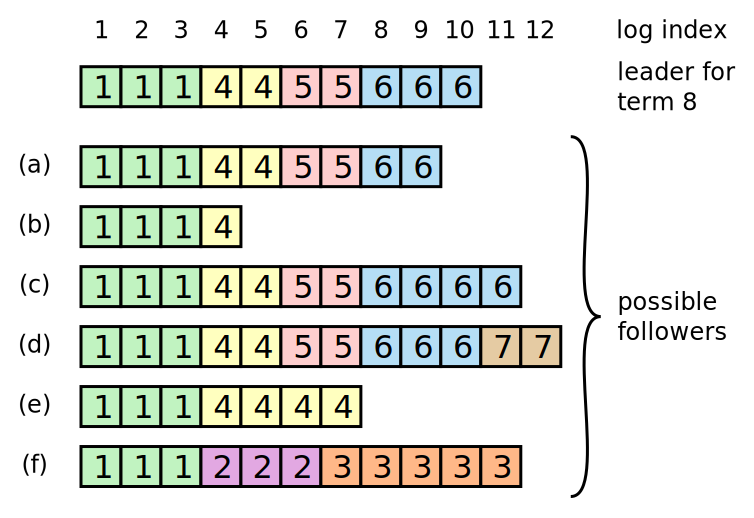
\includegraphics[scale=.50]{basicraft/diverge2}
\vcaption[log inconsistencies]{
When the leader at the top comes to power, it is possible that
any of scenarios (a--f) could occur in follower logs. Each box
represents one log entry; the number in the box is
its term. A follower may be missing entries (a--b), may have extra
uncommitted entries (c--d), or both (e--f). For example, scenario (f)
could occur if that server was the leader for term~2, added several entries
to its log, then crashed before committing any of them; it
restarted quickly, became leader for term 3, and added a few more
entries to its log; before any of the entries in either term 2 or term 3
were committed, the server crashed again and remained down for several terms.
}
\label{fig:basicraft:diverge}
\end{figure}

To bring a follower's log into consistency with its own,
the leader must find the latest log entry where the two logs agree,
delete any entries in the follower's log after that point,
and send the follower all of the leader's entries after that point.
All of these actions happen in response to the consistency check performed
by AppendEntries RPCs.
The leader maintains a \emph{nextIndex} for each follower, which
is the index of the next log entry the leader will send to that
follower. When a leader first comes to power, it initializes all nextIndex values
to the index just after the last one in its log (11 in
Figure~\ref{fig:basicraft:diverge}).
If a follower's log is inconsistent with the leader's, the AppendEntries
consistency check will fail in the next AppendEntries RPC.
After a rejection, the leader decrements the follower's nextIndex
and retries the AppendEntries
RPC. Eventually the nextIndex will reach a point where the leader and
follower logs match.
When this happens, AppendEntries will
succeed, which removes any conflicting entries in the follower's
log and appends
entries from the leader's log (if any). Once AppendEntries succeeds, the
follower's log is consistent with the leader's, and it will remain that way
for the rest of the term.

Until the leader has discovered where it and the follower's logs match,
the leader can send AppendEntries with no entries (like heartbeats) to
save bandwidth. Then, once the matchIndex immediately precedes the nextIndex,
the leader should begin to send the actual entries.

If desired, the protocol can be optimized to reduce the number of rejected
AppendEntries RPCs.  For example, when rejecting an AppendEntries request, the
follower can include the term of the conflicting entry
and the first index it stores for that term. With this
information, the leader can decrement nextIndex to bypass all of the conflicting
entries in that term; one AppendEntries RPC will be required for each term
with conflicting entries, rather than one RPC per entry.
Alternatively, the leader can use a binary search approach to find
the first entry where the follower's log differs from its own; this has
better worst-case behavior.
In practice, we
doubt these optimizations are necessary, since failures happen infrequently and
it is unlikely that there will be many inconsistent entries.

With this mechanism, a leader does not need to take any special actions
to restore log consistency when it comes to power. It just begins normal
operation, and the logs automatically converge in response to
failures of the AppendEntries consistency check.
A leader never overwrites or deletes entries in its own log (the Leader
Append-Only Property in Figure~\ref{fig:basicraft:properties}).

This log replication mechanism exhibits the desirable consensus properties
described in Section~\ref{motivation:problem}: \name{} can accept, replicate, and
apply new log entries as long as a majority of the servers are up;
in the normal case a new entry can be replicated with a single round
of RPCs to a majority of the cluster;
and a single slow follower will not impact performance.
The log replication algorithm is also practical to implement, since
AppendEntries requests are manageable in size (leaders never need to
send more than one entry in a single AppendEntries request to make
progress). Some other consensus algorithms are described as
sending entire logs over the network; this places a burden on the
implementer to develop optimizations required for a practical
implementation.

\section{Safety}
\label{basicraft:safety}

The previous sections described how \name{} elects leaders and
replicates log entries. However, the mechanisms described so far are not
quite sufficient to ensure that each state machine executes exactly the
same commands in the same order. For example, a follower might be
unavailable while the leader commits several log entries, then it
could be elected leader and overwrite these entries with new ones;
as a result, different state machines might execute different command
sequences.

This section completes the \name{} algorithm by adding a restriction
on which servers may be elected leader. The restriction ensures that the leader
for any given term contains all of the entries committed in previous
terms (the Leader Completeness Property from Figure~\ref{fig:basicraft:properties}).
Given the election restriction, we then make the rules for commitment
more precise. Finally, we present a proof sketch for the Leader
Completeness Property and show how it leads to correct
behavior of the replicated state machine.

\subsection{Election restriction}

In any leader-based consensus algorithm, the leader must eventually store
all of the committed log entries. In some consensus algorithms, such
as Viewstamped Replication~\cite{Liskov:2012},
a leader can be elected even if it doesn't initially contain all of the
committed entries. These algorithms contain additional mechanisms to identify
the missing entries and transmit them to the new leader, either during the
election process or shortly afterwards. Unfortunately, this results in
considerable additional mechanism and complexity. \name{} uses a simpler
approach where it guarantees that all the committed entries from previous
terms are present on each new leader from the moment of its election,
without the need to transfer those entries to the leader. This means
that log entries only flow in one direction, from leaders
to followers, and leaders never overwrite existing entries in their logs.

\begin{figure}
\centering
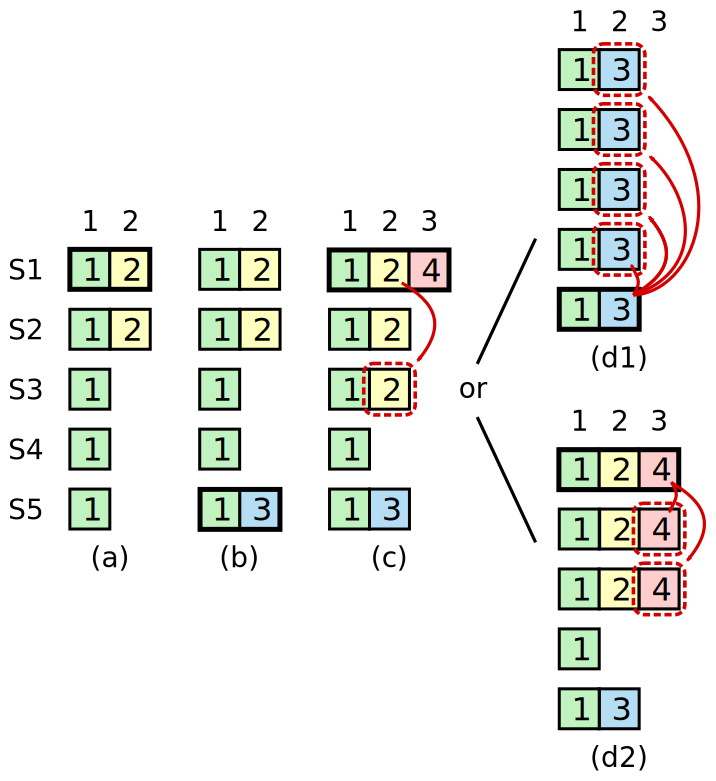
\includegraphics[scale=.50]{basicraft/oldTermCommit}
\vcaption[commitment rule]{
A time sequence showing why a leader cannot determine commitment
using log entries from older terms. In (a) S1 is leader and
partially replicates the log entry at index 2. In (b) S1 crashes;
S5 is elected leader for term 3 with votes from S3,
S4, and itself, and accepts a different entry at log index 2.
In (c) S5 crashes; S1 restarts, is elected leader, and continues
replication. At this point, the log entry from term 2 has been replicated
on a majority of the servers, but it is not committed. If S1 crashes
as in (d1), S5 could be elected leader (with votes from S2, S3,
and S4) and overwrite the entry with its own entry from term 3.
However, if S1 replicates an entry from its current term on a
majority of the servers before crashing, as in (d2), then this entry is
committed (S5 cannot win an election). At this point all preceding
entries in the log are committed as well.
}
\label{fig:basicraft:oldTermCommit}
\end{figure}

\name{} uses the voting process to prevent a candidate from winning
an election unless its log contains all committed entries. A candidate
must contact a majority of the cluster in order to be elected, which
means that every committed entry must be present in at least one of
those servers. If the candidate's log is at least as up-to-date as
any other log in that majority (where ``up-to-date'' is defined
precisely below), then it will hold all the committed entries.
The RequestVote RPC implements this restriction: the RPC includes
information about the candidate's log, and the voter denies
its vote if its own log is more up-to-date than that of the candidate.

\name{} determines which of two logs is more up-to-date by comparing
the index and term of the last entries in the logs. If
the logs have last entries with different terms, then the log with
the later term is more up-to-date. If the logs end with the same term,
then whichever log is longer is more up-to-date.

\subsection{Committing entries from previous terms}
As described in Section~\ref{basicraft:logreplication}, a leader knows
that an entry from its current term is committed once that entry
is stored on a majority of the servers. If a leader crashes
before committing an entry, future leaders will attempt to finish
replicating the entry. However, a leader cannot
immediately conclude that an entry from a previous term is
committed once it is stored on a majority of servers.
Figure~\ref{fig:basicraft:oldTermCommit}
illustrates a situation where an old log entry is stored on a
majority of servers, yet can still be overwritten by a future leader.

To eliminate problems like the one in
Figure~\ref{fig:basicraft:oldTermCommit}, Raft never commits log entries
from previous terms by counting replicas. Only log entries
from the leader's current term are committed by counting replicas;
once an entry from the current term has been committed in this way,
then all prior entries are committed
indirectly because of the Log Matching Property. There are some
situations where a leader could safely conclude
that an older log entry is committed (for example, if that entry is stored
on every server), but Raft takes a more conservative approach
for simplicity.

Raft incurs this extra complexity in the commitment rules because
log entries retain their original term numbers when a leader
replicates entries from previous terms. In other consensus algorithms,
if a new leader re-replicates entries from prior ``terms'',
it must do so with its new ``term number''. Raft's
approach makes it easier to reason about log entries, since they
maintain the same term number over time and across logs. In
addition, new leaders in Raft
send fewer log entries from previous terms than in other algorithms,
since other algorithms must send redundant log entries to renumber them
before they can be committed; however, this may not be very
important in practice, since leader changes should be rare.

\subsection{Safety argument}
\label{basicraft:safety:argument}

\newcommand\leaderT{$\textrm{leader}_\textrm{T}$}
\newcommand\leaderU{$\textrm{leader}_\textrm{U}$}

Given the complete Raft algorithm, we can now argue
more precisely that the Leader Completeness Property holds
(this argument is based on the safety proof; see
Chapter~\ref{correctness}).
We assume that the Leader Completeness Property
does not hold, then we prove a contradiction.
Suppose the leader for term T (\leaderT{}) commits a log entry from
its term, but that log entry is not stored by the leader of some
future term. Consider the smallest term U $>$ T whose leader (\leaderU{})
does not store the entry.

\begin{figure}
\centering
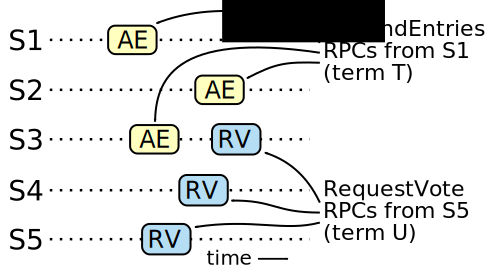
\includegraphics[scale=.50]{basicraft/safety2}
\vcaption[existence of voter in safety argument]{
If S1 (leader for term T) commits a new log entry from its term,
and S5 is elected leader for a later term U, then
there must be at least one server (S3) that accepted the log entry
and also voted for S5.
}
\label{fig:basicraft:safety2}
\end{figure}


\begin{enumerate}

\item The committed entry must have been absent from \leaderU{}'s log
at the time of its election (leaders never delete or overwrite entries).

\item \leaderT{} replicated the entry on a majority of the
cluster, and \leaderU{} received votes from a majority of
the cluster. Thus, at least one server (``the voter'') both accepted
the entry from \leaderT{} and voted for \leaderU{}, as shown
in Figure~\ref{fig:basicraft:safety2}. The voter is key to reaching a
contradiction.

\item  The voter must have accepted the committed entry from \leaderT{}
\emph{before} voting for \leaderU{}; otherwise it would have rejected
the AppendEntries request from \leaderT{} (its current term would
have been higher than T).

\item The voter still stored the entry when it voted for
\leaderU{}, since every intervening leader contained
the entry (by assumption), leaders never remove entries, and followers
only remove entries if they conflict with the leader.

\item The voter granted its vote to \leaderU{}, so \leaderU{}'s log must
have been as up-to-date as the voter's. This leads to one of two
contradictions.

\item First, if the voter and \leaderU{} shared the same last log term,
then \leaderU{}'s log must have been at least as long as the voter's,
so its log contained every entry in the voter's log. This is a contradiction,
since the voter contained the committed entry and \leaderU{} was assumed
not to.

\item Otherwise, \leaderU{}'s last log term must have been larger than
the voter's.
Moreover, it was larger than T, since the voter's last log term was at
least T (it contains the committed entry from term T). The earlier
leader that created \leaderU{}'s last log entry must have contained
the committed entry in its log (by assumption).
Then, by the Log Matching Property, \leaderU{}'s log must also contain
the committed entry, which is a contradiction.

\item This completes the contradiction. Thus, the leaders of all terms
greater than T must contain all entries from term T that are committed
in term T.

\item The Log Matching Property guarantees that future leaders
will also contain entries that are committed indirectly, such as
index 2 in Figure~\ref{fig:basicraft:oldTermCommit}(d2).

\end{enumerate}

Given the Leader Completeness Property, we can prove the State Machine
Safety Property from Figure~\ref{fig:basicraft:properties}, which states that
if a server has applied a log entry at a given index to its state
machine, no other server will ever apply a different log entry for the
same index.
At the time a server applies a log entry to its state machine, its log
must be identical to the leader's log up through that entry, and the
entry must be committed. Now consider the lowest term
in which any server applies a given log index; the Leader Completeness Property
guarantees that the leaders for all higher terms will store that same log
entry, so servers that apply the index in later terms will apply the same
value. Thus, the State Machine Safety Property holds.

Finally, \name{} requires servers to apply entries in log index order.
Combined with the State Machine Safety Property, this means that all
servers will apply exactly the same set of log entries to their state
machines, in the same order.

\section{Follower and candidate crashes}
Until this point we have focused on leader failures.
Follower and candidate crashes are much simpler to handle than leader
crashes, and they are both handled in the same way.
If a follower or candidate crashes (or the network link between it and
the leader fails), then future RequestVote and AppendEntries
RPCs sent to it will fail. Raft handles these failures by
retrying indefinitely;
if the crashed server restarts, then the RPC will complete
successfully.
If a server crashes after
completing an RPC but before responding, then it will receive the same
RPC again after it restarts. Raft RPCs have the same effect if repeated,
so this causes no harm. For example, if a follower receives an
AppendEntries request that includes log entries already present in
its log, it ignores those entries in the new request.

\section{Persisted state and server restarts}

Raft servers must persist enough information to stable storage to
survive server restarts safely. In particular, each server persists its
current term and vote; this is necessary to prevent the server from
voting twice in the same term or replacing log entries from a newer
leader with those from a deposed leader. Each server also persists new
log entries before they are counted towards the entries' commitment;
this prevents committed entries from being lost or ``uncommitted'' when
servers restart.

Other state variables are safe to lose on a restart, as they can all be
recreated.
The most interesting example is the commit index, which can safely be
reinitialized to zero on a restart. Even if every server restarts at the
same time, the commit index will only temporarily lag behind its true
value. Once a leader is elected and is able to commit a new entry, its
commit index will advance, and it will quickly propagate this commit
index to its followers.

The state machine can either be volatile or persistent. A volatile state
machine must be recovered after restarts by reapplying log entries
(after applying the latest snapshot; see Chapter~\ref{compaction}). A
persistent state machine, however, has already applied most entries
after a restart; to avoid reapplying them, its \emph{last applied} index
must also be persistent.

If a server loses any of its persistent state, it cannot safely rejoin
the cluster with its prior identity. Such a server can
usually be added back into the cluster with a new identity by invoking a
cluster membership change (see Chapter~\ref{membership}). If a majority
of the cluster loses its persistent state, however, log entries may be
lost and progress on cluster membership changes will not be possible; to
proceed, a system administrator would need to admit the possibility of
data loss.

\section{Timing and availability}
\label{basicraft:timing}

One of our requirements for \name{} is that safety must not depend
on timing: the system must not produce incorrect results just because
some event happens more quickly or slowly than expected. However,
availability (the ability of the system to respond to clients in a
timely manner) must
inevitably depend on timing. For example, if message exchanges take
longer than the typical time between server crashes, candidates will
not stay up long enough to win an election; without a steady leader,
\name{} cannot make progress.

Leader election is the aspect of \name{} where timing is most
critical. \name{} will be able to elect and maintain a steady
leader when the system satisfies the following
\emph{timing requirement}:
\begin{equation*}
\mathit{broadcastTime} \ll \mathit{electionTimeout} \ll \mathit{MTBF}
\end{equation*}
In this inequality \emph{broadcastTime} is the average time it takes a
server to send RPCs in parallel to every server in the cluster and receive
their responses; \emph{electionTimeout} is the election timeout described
in Section~\ref{basicraft:leaderelection}; and \emph{MTBF} is the
mean (average) time between failures for a
single server. The broadcast time should be an order of magnitude less than the
election timeout so that leaders can reliably send the heartbeat messages
required to keep followers from starting elections; given the randomized
approach used for election timeouts, this inequality also makes split votes
unlikely. 
The election timeout should be a few orders of magnitude less than MTBF
so that the system
makes steady progress. When the leader crashes, the system will be
unavailable for roughly the election timeout; we would like this to
represent only a small fraction of overall time.

The broadcast time and MTBF are properties of the underlying system, while
the election timeout is something we must choose. \name{}'s RPCs typically
require the recipient to persist information to stable storage, so the
broadcast time may range from \SIrange{0.5}{20}{\milli\second},
depending on storage
technology. As a result, the election
timeout is likely to be somewhere between
\SIrange{10}{500}{\milli\second}.
Typical server MTBFs are several months or more, which
easily satisfies the timing requirement.
Chapter~\ref{leaderelection} explores how to set the election timeout
and its impact on availability and leader election performance in more
detail.

\section{Leadership transfer extension}
\label{basicraft:leadershiptransfer}

This section describes an optional extension to Raft that allows one
server to transfer its leadership to another. Leadership transfer could
be useful in two types of situations:
%
\begin{enumerate}
%
\item Sometimes the leader must step down. For example, it may
need to reboot for maintenance, or it may be removed from the cluster
(see Chapter~\ref{membership}). When it steps down, the cluster will be
idle for an election timeout until another server times out and wins an
election. This brief unavailability can be avoided by having the leader
transfer its leadership to another server before it steps down.
%
\item In some cases, one or more servers may be more suitable to lead
the cluster than others. For example, a server with high load would not
make a good leader, or in a WAN deployment, servers in a primary
datacenter may be preferred in order to minimize the latency between
clients and the leader. Other consensus algorithms may be able
to accommodate these preferences during leader election, but Raft needs
a server with a sufficiently up-to-date log to become leader, which
might not be the most preferred one. Instead, a leader in Raft
can periodically check to see whether one of its available followers
would be more suitable, and if so, transfer its leadership to that
server. (If only human leaders were so graceful.)
%
\end{enumerate}

To transfer leadership in Raft, the prior leader sends its log entries to
the target server, then the target server runs an election without
waiting for an election timeout to elapse.
The prior leader thus ensures that the target server has all committed
entries at the start of its term, and, as in normal elections, the
majority voting guarantees the safety properties (such as the Leader
Completeness Property) are maintained. The following steps describe the
process in more detail:
%
\begin{enumerate}
%
\item The prior leader stops accepting new client requests.
%
\item The prior leader fully updates the target server's log to match
its own, using the normal log replication mechanism described in
Section~\ref{basicraft:logreplication}.
%
\item The prior leader sends a \emph{TimeoutNow} request to the target
server. This request has the same effect as the target server's election
timer firing: the target server starts a new election (incrementing its
term and becoming a candidate).
%
\end{enumerate}
%
Once the target server receives the TimeoutNow request, it is highly
likely to start an election before any other server and become leader in
the next term. Its next message to the prior leader will include its new
term number, causing the prior leader to step down. At this point,
leadership transfer is complete.

It is also possible for the target server to fail; in this case, the
cluster must resume client operations. If leadership transfer does not
complete after about an election timeout, the prior leader aborts the
transfer and resumes accepting client requests. If the prior leader was
mistaken and the target server is actually operational, then at worst
this mistake will result in an extra election, after which client
operations will be restored.

This approach preserves safety by operating within the normal
transitions of a Raft cluster. For example, Raft already guarantees
safety even when clocks run at arbitrary speeds; when the target server
receives a TimeoutNow request, it is equivalent to the target server's
clock jumping forwards quickly, which is safe. However, we have not currently
implemented or evaluated this leadership transfer approach.
